% !TEX TS-program = XeLaTeX
% !TEX encoding = UTF-8 Unicode

\chapter{实现与测试}
\label{chap07}
\defaultfont

\section{系统环境}

\subsection{硬件环境}

\begin{enumerate}
    \item CPU:Intel(R) Core(TM) i7-7700HQ CPU @ 2.80GHz   2.80 GHz
    \item 内存:16.0 GB
    \item 硬盘容量:500GB
\end{enumerate}

\subsection{软件环境}

\begin{enumerate}
    \item 操作系统:Windows 10 家庭中文版(20H2)作为编辑环境+ WSL2(Ubuntu 20.04)作为开发环境
    \item 数据库:mysql Ver 8.0.23-0ubuntu0.20.04.1 for Linux on x86\_64 (Ubuntu)
    \item 客户端:主流浏览器
\end{enumerate}


\section{持久化}
\subsection{Spring Date \& JPA Hibernate}

\begin{enumerate}
    \item 使用“逻辑模型工具”(例如Navicat Data Module 3)建立模型。
    \item 将模型同步至数据库
    \item 使用IDEA持久化工具生成实体类
    \item 根据逻辑模型为实体类添加注解(实现级联关系)
\end{enumerate}

关键问题如下:

\begin{enumerate}
    \item 多对一,一对多关系实现\\
          这种关系一共有四种实现方式
          \begin{enumerate}
              \item 单向\lstinline[language = Java]| @OneToMany |绑定
              \item 带有\lstinline[language = Java]| @JoinColumn |的单向\lstinline[language = Java]| @OneToMany |绑定
              \item 双向\lstinline[language = Java]| @OneToMany , @ManyToOne|绑定
              \item 不带有\lstinline[language = Java]| ManyToOne |的双向绑定
          \end{enumerate}
          本系统采用第三种方式
          \begin{lstlisting} [language = Java]
    public class A { //  一方
        ...
        @OneToMany(...)
        private List<B> bs;
        ...
    }
    public class B { // 多方
        @ManyToOne
        @JoinColumn(name = "a_id", referencedColumnName = "id")
        private A a;
    }
\end{lstlisting}
    \item 级联更新
          \begin{enumerate}
              \item 在“一方”(A)中 \lstinline[language = Java]| @OneToMany(cascade = CascadeType.ALL) |
              \item "深拷贝"A中的 \lstinline[language = Java]| BCopy = List<B> |
              \item 清空A中的 \lstinline[language = Java]| List<B> |
              \item \lstinline[language = Java]| BRepository.deleteAll(BCopy) |
              \item \lstinline[language = Java]| ARepository.save(A) |
          \end{enumerate}
    \item 级联查询
          \begin{enumerate}
              \item Dao层:继承JpaSpecificationExecutor
                    \begin{lstlisting} [language = Java]
    public interface ARepository extends 
        JpaRepository<A, Integer>, 
        JpaSpecificationExecutor<AEntity> // 注意这里
\end{lstlisting}
              \item Service层使用:
                    \begin{lstlisting} [language = Java]
    aRepository.findAll(new Specification<A>() {
        @Override
        // Hibernate根据此方法生成过滤语句
        public Predicate toPredicate(
            Root<UnfinishedPlanEntity> root, 
            CriteriaQuery<?> query, 
            CriteriaBuilder criteriaBuilder) {
          // 实现逻辑
        }
    })             
\end{lstlisting}
                    涉及的重要的类:
                    \begin{enumerate}
                        \item \lstinline[language = Java]| javax.persistence.criteria.Path |:通过实体类属性名获取字段值
                        \item \lstinline[language = Java]| javax.persistence.criteria.Join |:通过实体类属性名级联
                        \item \lstinline[language = Java]| javax.persistence.criteria.CriteriaBuilder |:拼接生成过滤
                    \end{enumerate}
          \end{enumerate}
\end{enumerate}

\section{登陆\&验证授权模块}

\subsection{JWT优势}

随着Web应用规模的逐渐扩大,传统的基于Session和cookie的身份验证技术逐渐显现出它的弊端。
随着服务器的不断增加,由于多个请求可以被分发给不同的服务器,那么此时,服务器该如何那些请求来自同一个用户,对此有两种解决方式
\begin{enumerate}
    \item 多个服务器之间同步用户状态,这样无论用户的请求分发到哪一个服务器,都可以操作用户状态
    \item 判断来自同一个用户的请求,将同一个用户的请求一直分发到同一个服务器
\end{enumerate}
很显然,无论是上述哪种方式,随着用户量的增长开销都会变得很大。
例如第一种方式可以使用会话复制实现,Sesson复制性能也会随着服务器的增加而急剧下降。\cite{.2019h}

JWT(JSON Web Token)的优势在于
\begin{enumerate}
    \item 将用户认证信息保存在客户端,减轻服务器的存储压力。
    \item 提供无状态的身份认证——不需要服务器端多端同步用户状态,利于分布式应用开发。\cite{.2019h}
\end{enumerate}


\subsection{使用JWT\&Spring Security 实现验证和授权}

\begin{figure}[h]
    \centering
    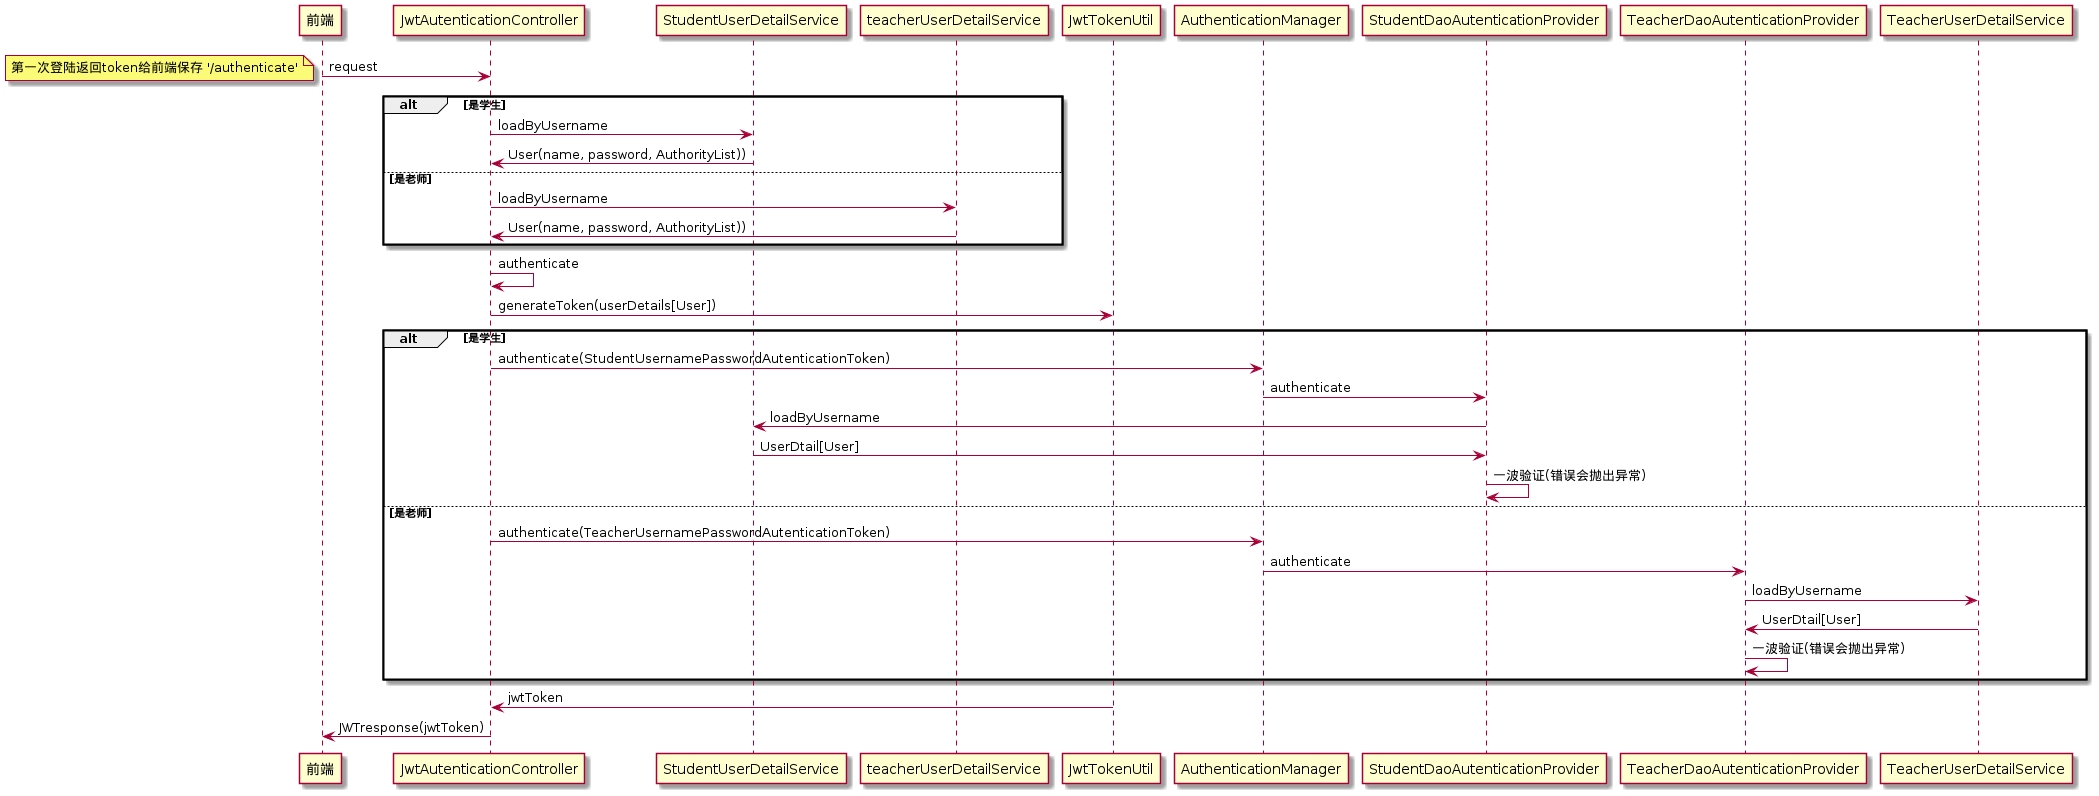
\includegraphics[scale = 0.3, angle = 90]{out/uml/时序图/时序图-authentication/时序图-authentication.png}
    \caption{\song\wuhao 登陆验证授权时序图}
\end{figure}

关键问题如下:
\begin{enumerate}
    \item 多用户表使用Spring Security\\
          验证授权涉及到的关键类(图\ref{SpringSecurity}):
          \begin{figure}[h]
              \centering
              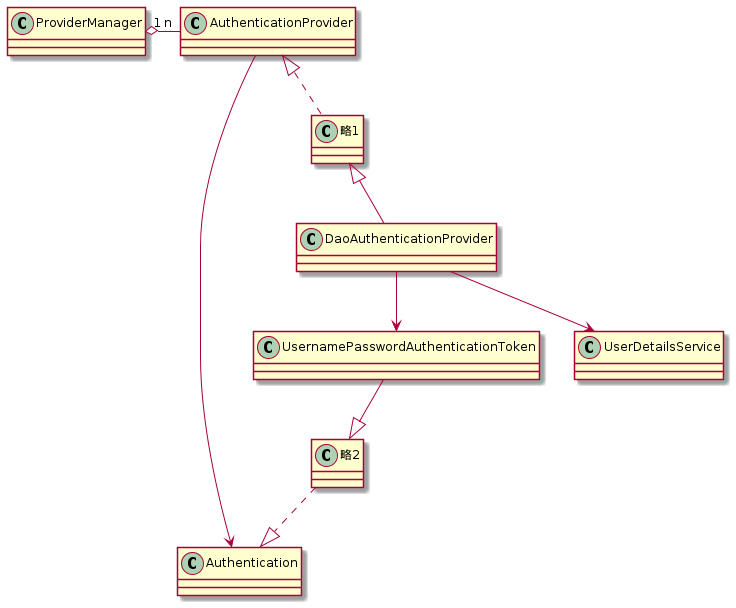
\includegraphics[scale = 0.5]{out/uml/类图/Spring Security/SpringSecurity验证/SpringSecurity验证.png}
              \caption{\song\wuhao Spring Security 验证授权关键类}
              \label{SpringSecurity}
          \end{figure}
          \begin{enumerate}
              \item \lstinline[language = Java]| Authentication |:用户认证信息。
              \item \lstinline[language = Java]| UsernamePasswordAuthenticationToken |:\lstinline[language = Java]| Authentication |的实现类,用于登陆验证,最为常用。
              \item \lstinline[language = Java]| AuthenticationProvider |:认证器,不同的\lstinline[language = Java]| AuthenticationProvider | 处理不同的 \lstinline[language = Java]| Authentication |
              \item \lstinline[language = Java]| DaoAuthenticationProvider |:\lstinline[language = Java]| AuthenticationProvider |的实现类,用于处理\lstinline[language = Java]| UsernamePasswordAuthenticationToken |
              \item \lstinline[language = Java]| ProviderManager |:用于管理\lstinline[language = Java]| AuthenticationProvider |
              \item \lstinline[language = Java]| UserDetailService |:为\lstinline[language = Java]| DaoAuthenticationProvider |提供从数据库查询用户的功能,用于做密码对比。
          \end{enumerate}
          多用户表配置Spring Security(图\ref{SpringSecurityMultiUser}):
          \begin{enumerate}
              \item 为不同用户建立各自的\lstinline[language = Java]| UserDetailService |
                    \begin{lstlisting} [language = Java]
    public class XXXUserDetialsService 
                implements UserDetailService
                \end{lstlisting}
                    ,各自的\lstinline[language = Java]| UserDetailService |从各自的数据库表中查询密码,提供给各自的\lstinline[language = Java]| DaoAuthenticationProvider |使用。
              \item 为不同用户建立各自的\lstinline[language = Java]| UsernamePasswordAuthenticationToken | \begin{lstlisting} [language = Java]
    public class XXXUPAuthToken 
                extends UsernamePasswordAuthenticationToken
              \end{lstlisting}
              \item 为不同用户建立各自的\lstinline[language = Java]| DaoAuthenticationProvider | \begin{lstlisting} [language = Java]
    public class XXXDaoAuthProvider 
                extends DaoAuthenticationProvider
              \end{lstlisting}
              \item 进行Security配置 \begin{lstlisting} [language = Java]
    @Configuration
    @EnableWebSecurity
    @EnableGlobalMethodSecurity(prePostEnabled = true)
    public class MySecurityConfig 
                extends WebSecurityConfigurerAdapter 
              \end{lstlisting}
                    需要的关键配置:\begin{enumerate}
                        \item 注入\lstinline[language = Java]| XXXAuthProvider |
                        \item 向\lstinline[language = Java]| AuthenticationManager |添加\lstinline[language = Java]| XXXAuthProvider |
                        \item 注入\lstinline[language = Java]| AuthenticationManager |
                    \end{enumerate}
          \end{enumerate}
          \begin{figure}[h]
              \centering
              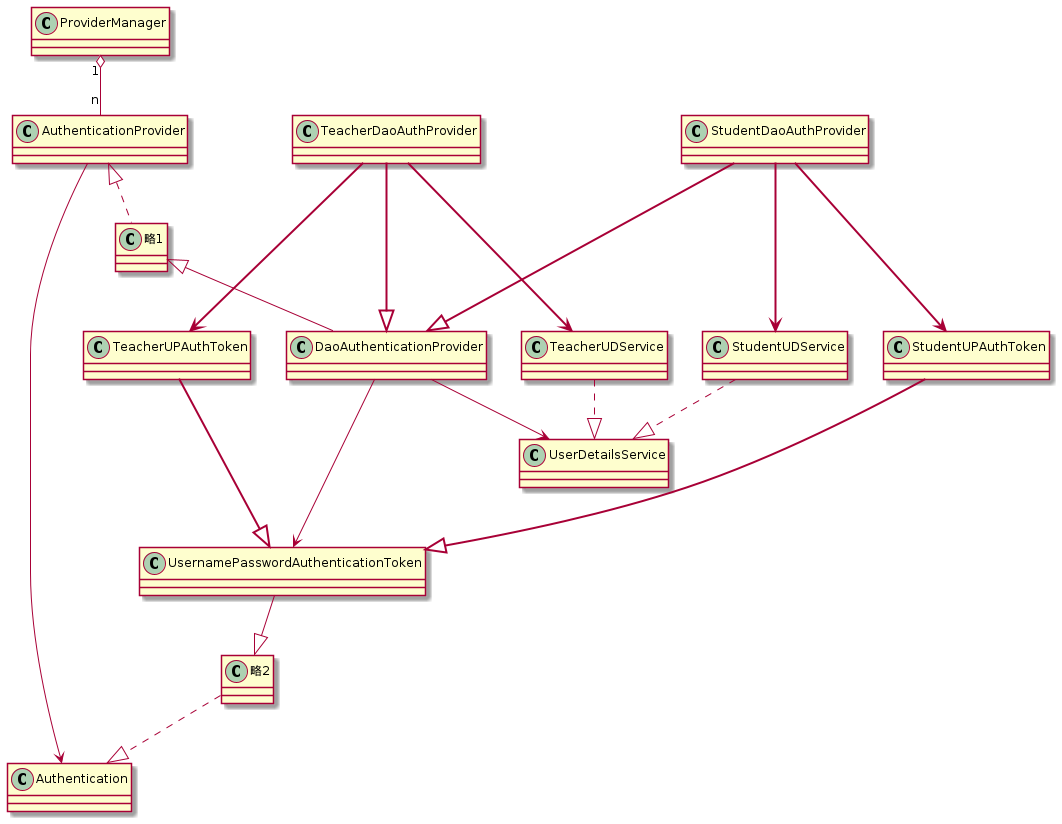
\includegraphics[scale = 0.35]{out/uml/类图/Spring Security/SpringSecurity多用户表验证/SpringSecurity多用户表验证.png}
              \caption{\song\wuhao SpringSecurity多用户表验证}
              \label{SpringSecurityMultiUser}
          \end{figure}
    \item CORS跨域问题\\
          CORS(Cross-origin resource sharing)——跨域资源共享,一种可以允许访问其他域名下的受限资源的机制。
          目前CORS的现行标准由WHATWG(Web Hypertext Application Technology Working Group)在网络浏览器中实现和测试。\\
          CORS-preflight request——预检请求,对于可能会对服务器造成副作用的请求(非简单请求),浏览器会先使用OPTIONS方法发送预检请求
          询问服务器是否允许此次跨域请求。\\
          简单请求需满足:
          \begin{enumerate}
              \item 请求方法:\lstinline[language = xml]| GET、POST、HEAD |
              \item 只使用了如下的安全首部字段,不得人为设置其他首部字段\begin{lstlisting} [language = Java]
    Accept
    Accept-Language
    Content-Language
    Content-Type 仅限以下三种
            text/plain
            multipart/form-data
            application/x-www-form-urlencoded
    HTML头部header field字段:
                DPR、Download、Save-Data、Viewport-Width、WIdth
              \end{lstlisting}
              \item 请求中的任意XMLHttpRequestUpload 对象均没有注册任何事件监听器;XMLHttpRequestUpload 对象可以使用 XMLHttpRequest.upload 属性访问
              \item 请求中没有使用 ReadableStream 对象
          \end{enumerate}
          CORS流程(图\ref{CORS-flow}):
          \begin{figure}[h]
              \centering
              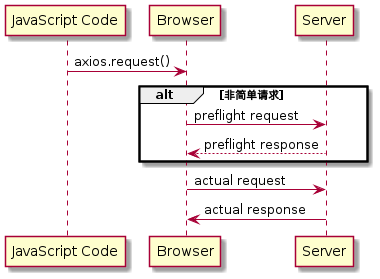
\includegraphics[scale = 0.6]{out/uml/时序图/CORS-flow/CORS-flow.png}
              \caption{\song\wuhao CORS流程}
              \label{CORS-flow}
          \end{figure}
          Spring Security 配置配置CORS:
          \begin{enumerate}
              \item 打开CORS \begin{lstlisting} [language = Java]
// MySecurityConfig.java
  protected void configure(HttpSecurity httpSecurity) 
                            throws Exception {
    httpSecurity..cors()
              \end{lstlisting}
              \item 配置配置CORS response
                    \begin{lstlisting} [language = Java]
// MySecurityConfig.java
@Bean
CorsConfigurationSource corsConfigurationSource() {
  CorsConfiguration configuration = new CorsConfiguration();
  configuration.addAllowedOrigin("*"); 
                // 应设置为前端服务器域名前缀
  configuration.setAllowedMethods(
              Arrays.asList("GET", "POST", "OPTION"));
  configuration.addAllowedHeader("*");
  // 允许的Header,起码需要允许 Access-Control-Allow-Origin
  UrlBasedCorsConfigurationSource source = 
                          new UrlBasedCorsConfigurationSource();
  source.registerCorsConfiguration("/**", configuration);
  return source;
}
          \end{lstlisting}
          \end{enumerate}
\end{enumerate}